\begin{figure}[p]
\centering
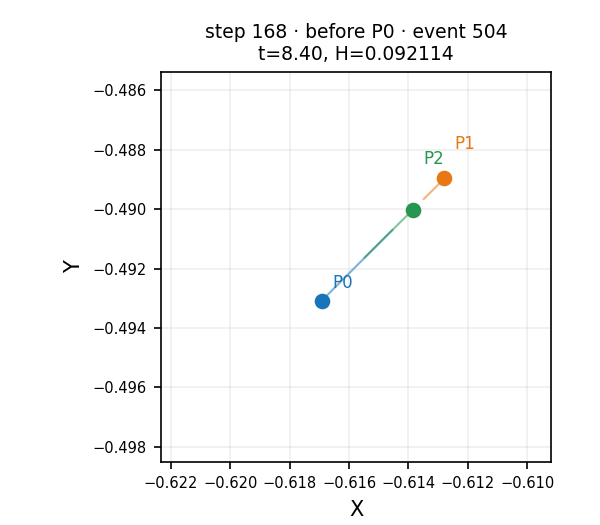
\includegraphics[width=0.485\linewidth,height=0.32\textheight,keepaspectratio]{figures/F04_0.png}
\hfill
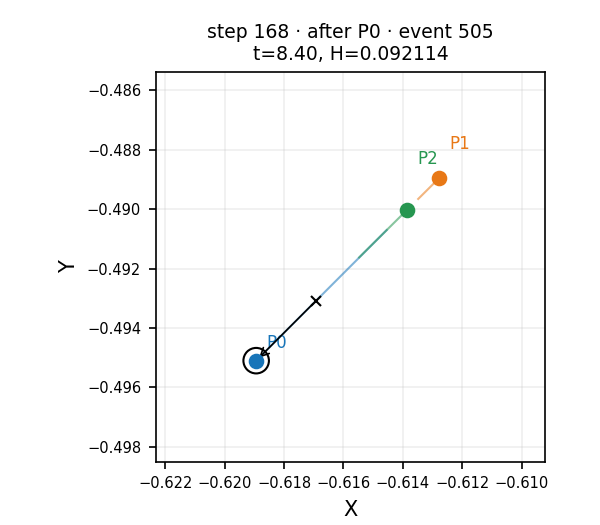
\includegraphics[width=0.485\linewidth,height=0.32\textheight,keepaspectratio]{figures/F04_1.png}
\par\medskip
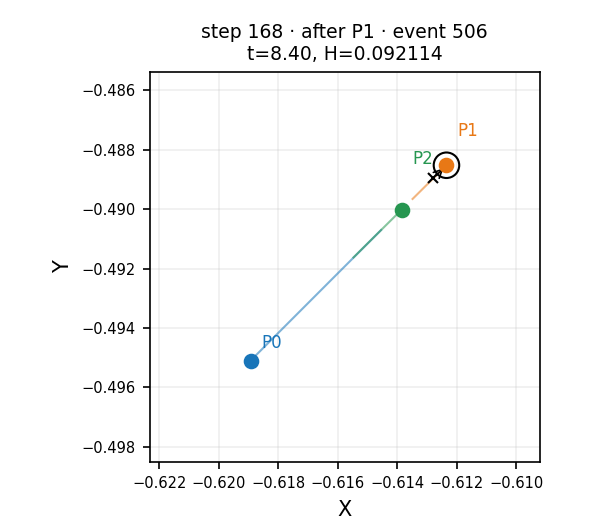
\includegraphics[width=0.485\linewidth,height=0.32\textheight,keepaspectratio]{figures/F04_2.png}
\hfill
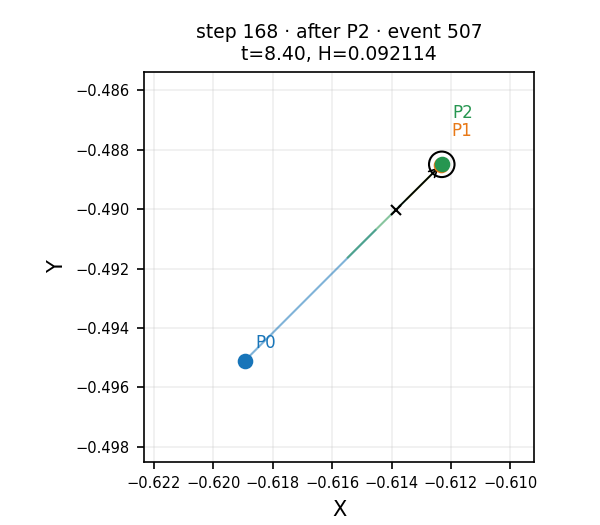
\includegraphics[width=0.485\linewidth,height=0.32\textheight,keepaspectratio]{figures/F04_3.png}
\par\medskip
\caption[A close pair during the central inspected sweep]{REPRODUCED / OBSERVED, editorial crop. Central row of the accepted near-contact sheet, arranged in reading order: event 504 before the sweep, then events 505,506,507. Source step 168 uses t=8.4. The local X/Y zoom makes the final near-overlap visible, while the saved velocities remain distinct. Table~\ref{tab:near 01} supplies the subsequent separation; no exact coincidence or interpolated meeting is asserted. \cite{replay01}}
\label{fig:F04}
\end{figure}
